% !TEX encoding = UTF-8 Unicode
\documentclass[a4paper,12pt]{article}

%-----------------------------------------Include package & set up some thing-----------------------------------------------
\usepackage{fontspec}
\setmainfont{Times New Roman} %set font
\usepackage{enumitem} % to format list
\usepackage{amsmath}
\usepackage{listings} % quote code
\usepackage{color}
\usepackage{hyperref} % cite hyperlink & bookmarks
\usepackage{setspace} % space
\usepackage{graphicx} % insert image
\usepackage{subcaption} % Multiple images
\usepackage{float}
\usepackage[margin=1in, footskip = 0.25in]{geometry} % Change margin with geometry package

\hypersetup{unicode, colorlinks,linkcolor=black, urlcolor=cyan} % format hyperlink and bookmarks

%Define title
\title{Báo cáo bài tập 4}
\author{1612174 - Phùng Tiến Hào - \href{mailto:tienhaophung@gmail.com}{tienhaophung@gmail.com}}
\date{07/04/2019}

%Code formatting with the listing package
\definecolor{codegreen}{rgb}{0,0.6,0}
\definecolor{codegray}{rgb}{0.3,0.3,0.3}
\definecolor{codepurple}{rgb}{0.58,0,0.82}
\definecolor{backcolour}{rgb}{0.92,0.92,0.88}

\lstdefinestyle{mystyle}{
	backgroundcolor=\color{backcolour},   
	commentstyle=\color{codegreen},
	keywordstyle=\color{blue},
	numberstyle=\tiny\color{codegray},
	stringstyle=\color{codepurple},
	basicstyle=\footnotesize,
	breakatwhitespace=false,         
	breaklines=true,                 
	captionpos=b,                    
	keepspaces=true,                 
	numbers=left,                    
	numbersep=5pt,                  
	showspaces=false,                
	showstringspaces=false,
	showtabs=false,                  
	tabsize=2,
	columns=fullflexible,
	frame=single
}

\lstset{style=mystyle}

\begin{document}
	\pagenumbering{gobble}
	\maketitle
	\newpage
	
	\doublespacing
	\tableofcontents
	\singlespace
	
	\newpage
	\pagenumbering{arabic}
	
	\section{Mô tả tổng quan dataset (nguồn gốc, mục đích nghiên cứu, tổng thể nghiên cứu, cách thu thập dữ liệu, cỡ mẫu, số lượng biến).}
	\begin{itemize}
		\item Nguồn gốc:
		Gelman and Hill phân tích dữ liệu sử dụng hồi quy và mô hình đa cấp /phân cấp của đại học Cambridge tại New York năm 2007
		
		\item Mục đích nghiên cứu:
		Khảo sát và phân tích các đánh giá của các học sinh về bạn khác giới của mình trong cuộc gặp gỡ 4 phút của trường Columbia 
		về việc tham dự sự kiện "SpeedDating".
		
		\item Tổng thể nghiên cứu:
		Những người tham dự sự kiện "SpeedDating" là học sinh của trường Columbia được chọn lọc bởi các trợ lý nghiên cứu.
		
		\item Cách thu thập dữ liệu:
		\begin{itemize}
			\item Lấy dữ liệu ngày đầu tiên của cuộc hội giữa người tham dự và bạn tình của họ
			\item Các cuộc gặp gỡ được chọn ngẫu nhiên và thời lượng 4 phút
			\item Sau đó, người tham dự đánh giá các thuộc tính trên thang điểm 1-10.
		\end{itemize}
		
		\item Cỡ mẫu: 276 quan sát
		\item Số lượng biến: 22 biến
		
	\end{itemize}
		
		
		
		
	\section{Chọn ra 5 biến quan tâm, trong đó có ít nhất 2 biến định tính và 2 biến định lượng. Mô tả sơ
		lược ý nghĩa 5 biến này và nêu lí do chọn.}
		
		\begin{enumerate}[label = {\alph*)}]
			\item Các biến định tính:\\
			\begin{itemize}
				\item DecisionMale (Yes/No): Quyết dịnh nam có muốn 1 ngày hẹn nào khác không?
				\item RaceF (Asian, Black,...): Chủng tộc của bạn nữ
				\item[\textrightarrow] Lý do: vì cái kết quả quan trọng nhất là bạn nam tham dự có muốn tiến đến cuộc hẹn hò 
				thật sự vào một ngày khác không. Thường con trai họ sẽ thích những người cùng chủng tộc với họ.
			\end{itemize}
			
			
			\item Các biến định lượng:\\
			\begin{itemize}
				\item AttractiveM (num): Nam đánh giá về sức quyến rũ của bạn nữ.
				\item LikeM (num): Mức độ thích của người nam đối với nữ.
				\item SincereM (num): Mam đánh giá về độ chân thành của nữ.
				\item[\textrightarrow] Lý do: Đây các yếu tố mang tính cảm tính để quyết định người nam có ấn tượng ban đầu tốt đối với người phụ nữ và ảnh hưởng đến DecisionMale.
			\end{itemize}
		\end{enumerate}
	
	\section{Phân tích thăm dò riêng từng biến đã chọn:}
		\footnote{Nên dùng attach(SpeedDating) để khỏi phải gõ \$ trước tên biến mỗi khi truy cập}
		\footnote{Nếu attach rồi thì phải detach(SpeedDating) khi đã dùng xong}
		\begin{enumerate}[label = {\alph*)}]
			\item Biến định tính:
				\begin{itemize}
					\item DecisionMale:\\
					
					\begin{lstlisting}[language = R]
					tab1 = table(DecisionMale) # Count so luong nam yes va no
					# Them total
					addmargins(tab1)
					> DecisionMale
					No Yes Sum 
					130 146 276
					
					prop.table(tab1) # Proportions
					> DecisionMale
					No       Yes 
					0.4710145 0.5289855 
					
					barplot(tab1) # Ve barchart
					\end{lstlisting}
						
						\begin{figure}[H]
							\centering
							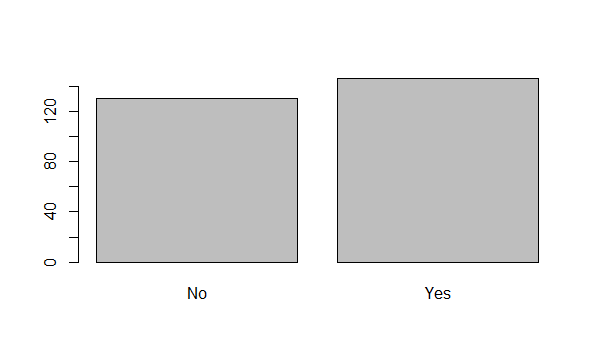
\includegraphics[width=\linewidth]{Images/Rplot01}
							\caption[]{DecisionMale barchar}
						\end{figure}
					
					NX: Tỉ lệ nam đồng ý nhiều hơn là không đồng ý. ($0.529 - 0.471 = 0.058$)
					
					\item RaceF:\\
						\begin{lstlisting}[language = R]
						tab2 = table(RaceF) #Count so luong nu cho tung chung toc
						# Them total
						addmargins(tab2)
						> RaceF
								Asian    Black Caucasian    Latino    Other       Sum 
						4       70       15       148       23        16      	   276
						
						prop.table(tab2) # Proportions
						> RaceF
										Asian      Black  Caucasian     Latino      Other 
						0.01449275 0.25362319 0.05434783 0.53623188 0.08333333 0.05797101
						
						barplot(tab2)
						\end{lstlisting}
						
						\begin{figure}[H]
							\centering
							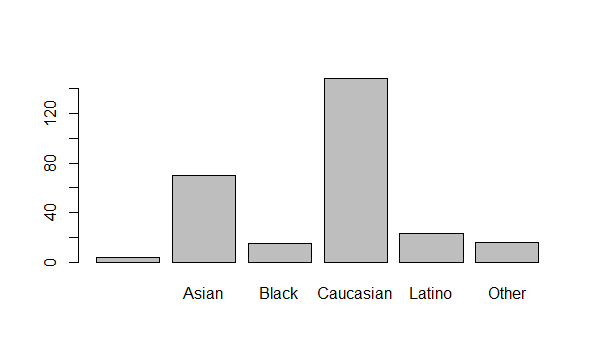
\includegraphics[width=\linewidth]{Images/Rplot}
							\caption[]{RaceF barchar}
						\end{figure}
						
						NX chung: Tỷ lệ nữ trắng nhiều nhất ($0.536$), tiếp đến là nữ châu Á ($0.254$).
						
						
				\end{itemize}
				
			\item Biến định lượng:\\
			
			
				Mặc dù trung bình (mean) thường được sử dụng để mô tả trọng tâm của phân phối nhưng nó lại rất nhạy cảm với ngoại lệ (outlier). Do đó, trung vị (median) được dùng thay thế vì ít chịu ảnh hưởng của outlier.
				
				
				Thêm vào đó, interquartile range (IQR): $IQR = Q_3 - Q_1$. Đây là đại lượng dùng để đo độ lan ra của dữ liệu (measure of spread) và ít bị ảnh hưởng bởi nhiễu.
				
				
				Thông thường, người ta sử dụng median kèm với IQR như là 1 measure of spread khi mà dữ liệu có nhiều nhiễu.
				
				
				\begin{itemize}
				\item  AttractiveM:\\
					\begin{lstlisting}[language = R]
						# AttractiveM
						five_num = summary(AttractiveM) # 5-number summary
						>
						  Min. 1st Qu.  Median    Mean 3rd Qu.    Max.    NA 
						1.000   5.000   7.000   6.687   8.000  10.000       3
						
						# Range:
						range = five_num[6] - five_num[1]; range
						> 9
						
						# Interquartile range
						IQR = five_num[5] - five_num[2]; IQR
						> 3
						
						# Detect outlier: smaller than Q1 - 1.5(IQR) or greater than Q3 + 1.5(IQR)
						(t1 <- five_num[2] - 1.5*IQR); (t2 <- five_num[5] + 1.5*IQR)
						> 0.5
						12.5
						
						# Dotplot de dem so luong cho tung diem tuong ung
						dotPlot(~AttractiveM, width = 1, cex = 0.35)
						# Ve histogram
						hist(AttractiveM)
						# Ve phan bo cua du lieu
						densityplot(AttractiveM)
						
					\end{lstlisting}
					
					\begin{figure}[H]
						\centering
						\begin{subfigure}[b]{0.8\linewidth}
							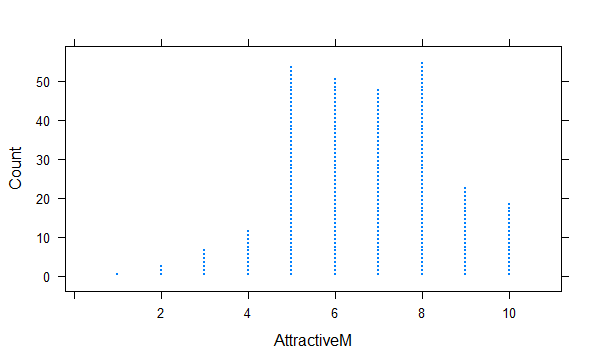
\includegraphics[width=\linewidth]{Images/dotplot1}
							\caption{Dotplot of AttractiveM}
						\end{subfigure}
						\begin{subfigure}[b]{0.4\linewidth}
							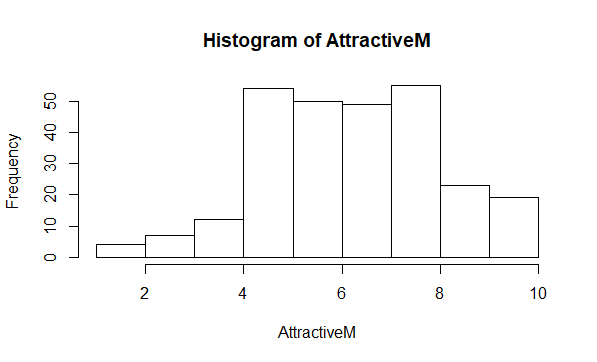
\includegraphics[width=\linewidth]{Images/Rplot2}
							\caption{Histogram of AttractiveM}
						\end{subfigure}
						\begin{subfigure}[b]{0.4\linewidth}
							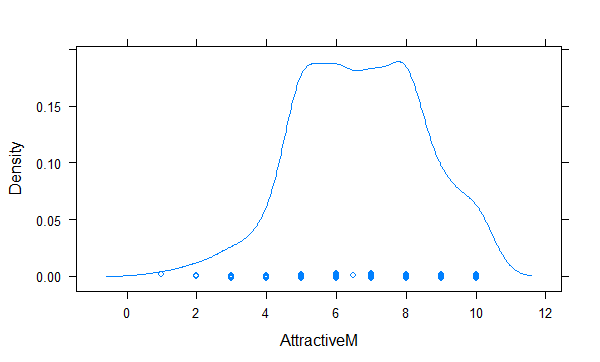
\includegraphics[width=\linewidth]{Images/denplot1}
							\caption{Density of AttractiveM}
						\end{subfigure}
						\label{fig:rplot2}
					\end{figure}
					
					
					\begin{itemize}
						\item Đồ thị có dạng "xấp xỉ" bell-shape, gần đối xứng hai bên.
						\item 25\% Nam đánh giá sức quyến rũ của bạn nữ ít nhất 1 - 5 điểm
						\item 50\% Nam đánh giá sức quyến rũ của bạn nữ trong khoảng 5 - 8 điểm
						\item 25\% Nam đánh giá sức quyến rũ của bạn nữ nhiều nhất từ 8 - 10 điểm
						\item Kết luận:
						\begin{itemize}
							\item 50\% Nam đánh giá sức quyến rũ của bạn nữ ít hơn 7 điểm.
							\item 50\% Nam đánh giá sức quyến rũ của bạn nữ trên 7 điểm.
						\end{itemize}
						\item Ta thấy $range = Max - Min = 9$, phân bố từ 1 - 10.
						\item Ta tính được interquartile range (IQR): $IQR = Q_3 - Q_1 = 3$.
						\item Dưa vào IQR, ta sẽ phát hiện được phạm vi phân bố của outliers:
						Nhỏ hơn $Q_1 - 1.5*IQR = 0.5$ hay lớn hơn $Q_3 + 1.5*IQR = 12.5$. Ta thấy rằng không có outlier nào lớn hơn 12.5 và cũng không có outlier nào bé hơn 0.5 trong dữ liệu.  Điều này cho thấy dữ liệu đã được thu thập rất tốt. 
					\end{itemize}
					
					
				\item LikeM:
					\begin{lstlisting}[language = R]
					# LikeM
					five_num = summary(LikeM) # 5-number summary
					> 
					Min. 1st Qu.  Median    Mean 3rd Qu.    Max.    NA 
					1.000   6.000   7.000   6.682   8.000  10.000       2
					
					# Range:
					range = five_num[6] - five_num[1]; range
					> 9
					
					# Interquartile range
					IQR = five_num[5] - five_num[2]; IQR
					> 2
					
					# Detect outlier: smaller than Q1 - 1.5(IQR) or greater than Q3 + 1.5(IQR)
					(t1 <- five_num[2] - 1.5*IQR); (t2 <- five_num[5] + 1.5*IQR)
					> 3
					11
					
					# Tim so luong cac doi tuong outlier
					# TH: < t1
					count(subset(SpeedDating, LikeM < t1))
					> 6
					
					# Dotplot de dem so luong cho tung diem tuong ung
					dotPlot(~LikeM, width = 1, cex = 0.35)
					# Ve histogram
					hist(LikeM)
					# Ve phan bo cua du lieu
					densityplot(LikeM)
					\end{lstlisting}
					
					\begin{figure}[H]
						\centering
						\begin{subfigure}[b]{0.8\linewidth}
							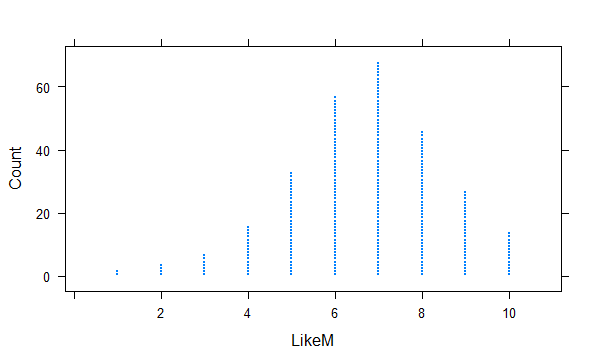
\includegraphics[width=\linewidth]{Images/dotplot2}
							\caption{Dotplot of LikeM}
						\end{subfigure}
						\begin{subfigure}[b]{0.4\linewidth}
							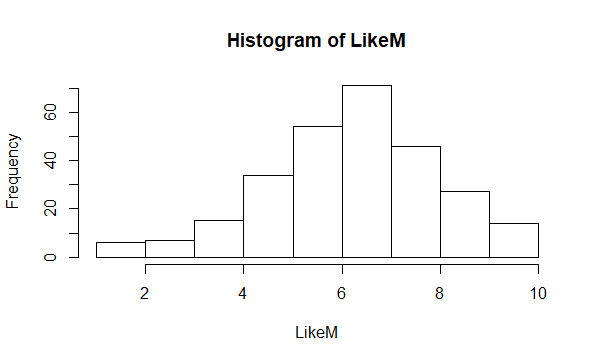
\includegraphics[width=\linewidth]{Images/Rplot3}
							\caption{Histogram of LikeM}
						\end{subfigure}
						\begin{subfigure}[b]{0.4\linewidth}
							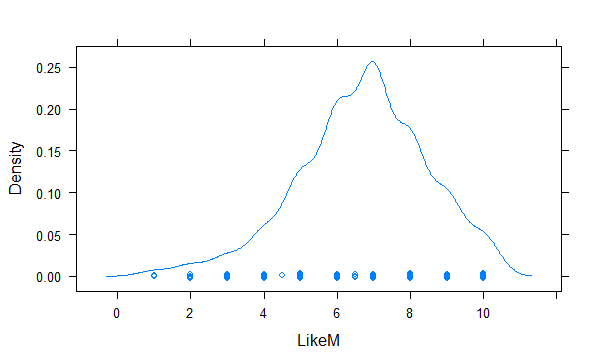
\includegraphics[width=\linewidth]{Images/denplot2}
							\caption{Density of LikeM}
						\end{subfigure}
						\label{fig:rplot3}
					\end{figure}
					
					\begin{itemize}
						\item Đồ thị có dạng bell-shape, gần đối xứng 2 bên
						\item 25\% mức độ thích thú của nam ít nhất 1 - 6 điểm 
						\item 50\% mức độ thích thú của nam trong khoảng 6 - 8 điểm
						\item 25\% mức độ thích thú của nam nhiều nhất từ 8 - 10 điểm
						\item Kết luận:
						\begin{itemize}
							\item 50\% mức độ thích thú của nam ít hơn 7 điểm.
							\item 50\% mức độ thích thú của nam trên 7 điểm.
						\end{itemize}
						\item Ta thấy $range = Max - Min = 9$, phân bồ từ 1 - 10.
						\item Ta tính được interquartile range (IQR): $IQR = Q_3 - Q_1 = 2$.
						\item Dưa vào IQR, ta sẽ phát hiện được phạm vi phân bố của outliers:
						Nhỏ hơn $Q_1 - 1.5*IQR = 3$ hay lớn hơn $Q_3 + 1.5*IQR = 11$. Ta thấy rằng có 6 outliers dưới 3 và không có outlier nào lớn hơn 11 trong dữ liệu.
					\end{itemize}
					
					
					
				\item SincereM:
					\begin{lstlisting}[language = R]
					# SincereM
					summary(SincereM) # 5-number summary
					>
					 Min. 1st Qu.  Median    Mean 3rd Qu.    Max.    NA 
					1.000   7.000   8.000   7.856   9.000  10.000       5
					
					# Range:
					range = five_num[6] - five_num[1]; range
					> 9
					
					# Interquartile range
					IQR = five_num[5] - five_num[2]; IQR
					> 2
					
					# Detect outlier: smaller than Q1 - 1.5(IQR) or greater than Q3 + 1.5(IQR)
					(t1<-five_num[2] - 1.5*IQR); (t2 <- five_num[5] + 1.5*IQR)
					> 4
					12
					
					# Tim so luong cac doi tuong outlier
					# TH: < t1
					count(subset(SpeedDating, LikeM < t1))
					> 13
					
					# Dotplot de dem so luong cho tung diem tuong ung
					dotPlot(~SincereM, width = 1, cex = 0.35)
					# Ve histogram
					hist(SincereM)
					# Ve phan bo cua du lieu
					densityplot(SincereM)
					\end{lstlisting}
					
					\begin{figure}[H]
						\centering
						\begin{subfigure}[b]{0.8\linewidth}
							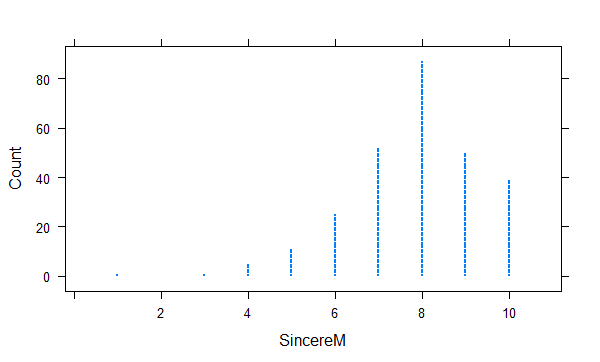
\includegraphics[width=\linewidth]{Images/dotplot3}
							\caption{Dotplot of SincereM}
						\end{subfigure}
						\begin{subfigure}[b]{0.4\linewidth}
							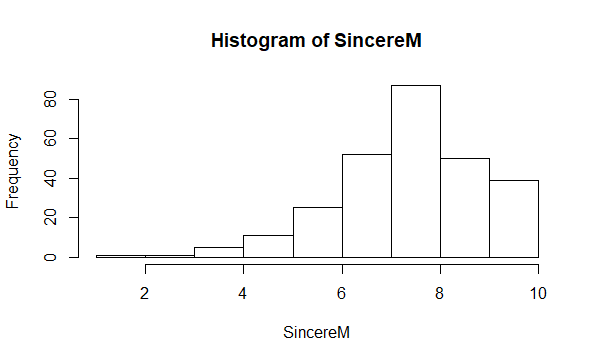
\includegraphics[width=\linewidth]{Images/Rplot4}
							\caption{Histogram of SincereM}
						\end{subfigure}
						\begin{subfigure}[b]{0.4\linewidth}
							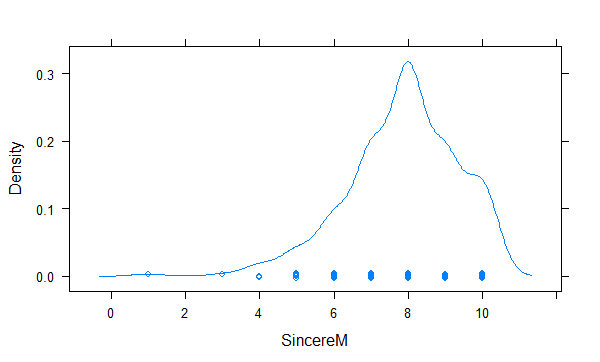
\includegraphics[width=\linewidth]{Images/denplot3}
							\caption{Density of SincereM}
						\end{subfigure}
						\label{fig:rplot4}
					\end{figure}
					
					
					\begin{itemize}
						\item Đồ thị hơi nghiêng về bên trái do đó $mean < median$ (7.856 < 8)
						\item 25\% nam đánh giá độ chân thành của nữ ít nhất 1 - 7 điểm
						\item 50\% nam đánh giá độ chân thành của nữ trong khoảng 7 - 9 điểm
						\item 25\% nam đánh giá độ chân thành của nữ nhiều nhất từ 9 - 10 điểm
						 
						\item Kết luận:
							\begin{itemize}
								\item 50\% nam đánh giá độ chân thành của nữ ít hơn 8 điểm.
								\item 50\% nam đánh giá độ chân thành của nữ trên 8 điểm.
							\end{itemize}
								\item Ta thấy $range = Max - Min = 9$, phân bồ từ 1 - 10.
							\item Ta tính được interquartile range (IQR): $IQR = Q_3 - Q_1 = 2$.
							\item Dưa vào IQR, ta sẽ phát hiện được phạm vi phân bố của outliers:
							Nhỏ hơn $Q_1 - 1.5*IQR = 4$ hay lớn hơn $Q_3 + 1.5*IQR = 12$. Ta thấy rằng có 13 outliers dưới 4 (khá nhiều) và không có outlier nào lớn hơn 12 trong dữ liệu.
					\end{itemize}
					
				
				NX cảm tính: Độ chân thành và sức quyến rũ của bạn nữ dễ ảnh hưởng đến DecisionM và LikeM của nam.
					
				\end{itemize}
				
		\end{enumerate}
	
	\section{Chọn ra 2 biến định tính (từ 5 biến quan tâm) và phân tích thăm dò quan hệ giữa chúng.}
	
	\underline{Chọn 2 biến định tính:} DecisionMale (Yes/No), RaceF (Asian, Black, Caucasian, Latino, or Other)\\
	
	
	\begin{lstlisting}[language = R]
	# 2 bien dinh tinh
	tab1 = table(DecisionMale, RaceF)
	# Them margin
	addmargins(tab1)
	
	>
	            RaceF
	DecisionMale     Asian Black Caucasian Latino Other Sum
			No    2    32     7        72      7    10 130
			Yes   2    38     8        76     16     6 146
			Sum   4    70    15       148     23    16 276
	
	# 2-way table
	# Ti le nam (yes/no) dieu kien chung toc nu (Asian, Black, ...)
	prop.table(tab1, margin = 1)
	
	>
	            RaceF
	DecisionMale                 Asian      Black  Caucasian     Latino      Other
			No  0.01538462 0.24615385 0.05384615 0.55384615 0.05384615 0.07692308
			Yes 0.01369863 0.26027397 0.05479452 0.52054795 0.10958904 0.04109589
	
	# Segmented barchart
	barplot(tab1, legend = TRUE)
	\end{lstlisting}
	
	\begin{figure}[H]
		\centering
		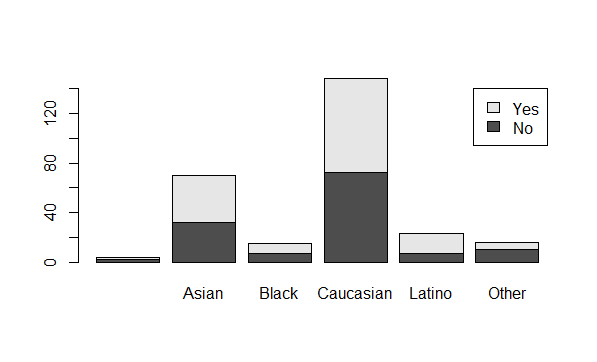
\includegraphics[width=0.7\linewidth]{Images/drplot}
		\caption{Segmented barchart of 2 categorial variables}
		\label{fig:drplot}
	\end{figure}
	
	
	\begin{itemize}
		\item Ta thấy rằng tỉ lệ phản hồi (no/yes) của nam đối với chủng tộc nữ da trắng (Caucasian) là cao nhất (0.553, 0.52). Tiếp đến là nữ châu Á (Asian) (0.246, 0.26).
		\item Tỉ lệ phẩn hồi "yes" và "no" đối với nữ da trắng:
		\begin{align*}
			p_{yes} &\approx 0.52 \\
			p_{no} &\approx 0.553 \\
		\end{align*}
		
		\item Tỉ lệ khác biệt (difference proportion) giữa tỉ lệ phản hồi "yes" và phản hồi "no" đối với nữ da trắng:
		$$p_{yes} - p_{no} = 0.52 -0.553 = -0.033$$
		\item[\textrightarrow] Tỷ lệ người nam phản hồi 'no' cao hơn phản hồi 'yes' đối với nữ da trắng 0.033.
		
		\item Tỷ lệ nam phản hồi "yes" đối với người da trắng cao hơn với người châu Á: $0.553 - 0.246 = 0.307$
		
		\item Từ bảng 2-way table, ta thấy rằng có 4 người nữ không có chủng tộc: 2 nhận phản hồi "yes" và 2 nhận phản hồi no "no". Đây là nhóm nhận được phản hồi ít nhất, cũng dễ hiểu vì trong nhóm này chỉ có duy nhất 4 người.
		
		NX: Người da trắng (Caucasian) và người da màu (Asian) nhận được sự phản hồi cao hơn các tộc còn lại.
	\end{itemize}
	
	\section{Chọn ra 1 biến định tính, 1 biến định lượng (từ 5 biến quan tâm) và phân tích thăm dò quan hệ giữa chúng.}
	\underline{Chọn 1 biến định tính và 1 biến định lượng:} DecisionMale (yes/no), AttractiveM (1-10)\\
	
	
	\begin{lstlisting}[language = R]
		# 1 quantitative and 1 categorical varibles
		# statistics for the quantitative variable within each category
		by(AttractiveM, DecisionMale, mean, na.rm=TRUE)
		>
		DecisionMale: No
		[1] 5.641732
		----------------- 
		DecisionMale: Yes
		[1] 7.59589
		
		# Tinh favorite statistics
		favstats(~AttractiveM | DecisionMale)
		>   
		DecisionMale	min	Q1	median	Q3	max     mean       sd   n missing
		1           No  	 1 	 5      5 	 6  	10 5.641732	 1.694877 127       3
		2          Yes  	 5 	 7      8 	 8  	10 7.595890	 1.357375 146       0
		
		# side-by-side boxplots
		boxplot(AttractiveM ~ DecisionMale, xlab = 'DecisionMale', ylab = 'AttractiveM')
	\end{lstlisting}
	
	\begin{figure}[H]
		\centering
		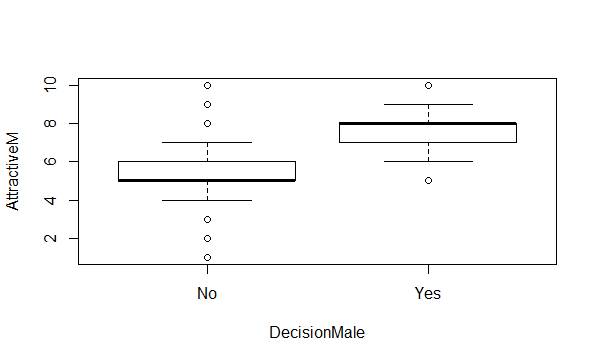
\includegraphics[width=0.8\linewidth]{Images/boxplot}
		\caption{Side-by-side boxplots}
		\label{fig:boxplot}
	\end{figure}
	
	\begin{itemize}
		\item Ở trường hợp phản hồi "no", Ta thấy median trùng với 1st quartile bằng 5.
		\item Ở trường hợp phản hồi "yes", ta thấy median trùng với 3rd quartile bằng 8.
		\item Do $se_{no} = 1.695 > se_{yes} = 1.357$ nên các outlier của phản hồi "no" xuất hiện nhiều hơn của phản hồi "yes". Điều này làm tần suất của dữ liệu trải dài đều từ 1 - 10.
		\item Ta thấy rằng có TH outlier bên phản hồi "no" có attractiveM = 10. Điều này khá bất thường. Còn bên phản hồi "yes" thì các outlier không đáng kể lắm, phân bố cũng gần IQR của dữ liệu.

		\item Thêm vào đó, ta thấy rằng mean của DecisionMale: No (5.641) < mean của DecisionMale: Yes (7.59). Do đó ta có thể nói mức điểm quyến rũ của phản hồi "yes" cao hơn của phản hồi "no".
		
		\item Đối với phản hồi "no", ta thấy rằng median < mean do có nhiều outlier trải dải từ 1-10. Ngược lại, phản hồi "yes" có median > mean do ít outlier hơn và phân bố của outlier cũng không quá xa IQR của dữ liệu.
		
		\item Interquartile range của phản hồi "yes" và "no" bằng nhau $(IQR = 1)$.
		
		\item Chúng ta thấy có 1 liến kết khi AttractiveM càng cao thì khả năng phản hồi yes cũng cao tuy rằng liên kết này không quá mạnh.
	\end{itemize}
	
	\section{Chọn ra 2 biến định lượng (từ 5 biến quan tâm) và phân tích thăm dò quan hệ giữa chúng.}
	\label{Cau6}
	\underline{Chọn 2 biến định lượng:} AttractiveM (1-10) và LikeM (1-10)\\
	
	
	\begin{lstlisting}[language=R]
		# 2 quantitative varibles
		# Summary statistics: correlation, regression line
		> cor(AttractiveM, LikeM, use = "complete.obs") # avoid missing value NA
		[1] 0.7240187
		
		> lm(LikeM~AttractiveM) # Linear regression for 2 varibles
		
		Call:
		lm(formula = LikeM ~ AttractiveM)
		
		Coefficients:
		(Intercept)  AttractiveM  
		1.9110       0.7139
		
		
		# Graphical display: scatterplot
		plot(AttractiveM, LikeM, main = "Scatter plot example", pch=19)
		# Add fit lines
		abline(lm(LikeM~AttractiveM), col="red") # regression line (y~x)
	\end{lstlisting}
	
	\begin{figure}[H]
		\centering
		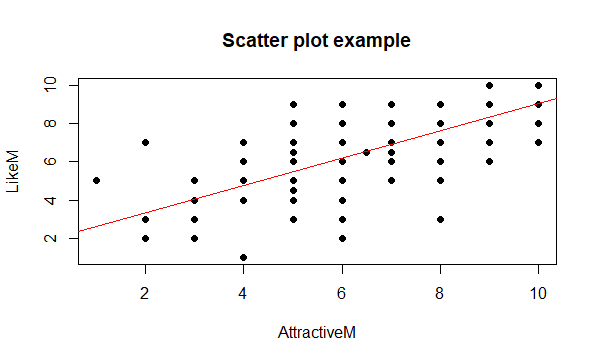
\includegraphics[width=0.8\linewidth]{Images/scatterplot}
		\caption{Scatterplot of 2 quantitative variables}
		\label{fig:scatterplot}
	\end{figure}
	
	\begin{itemize}
		\item Ta thấy rằng giữa 2 biến định lượng này có liên kết dương khá mạnh (positive association) $(r = 0.724)$ do đó nhìn chung khi AttractiveM tăng thì LikeM cũng tăng.
		\item Tuy rằng, có liên kết mạnh nhưng điều này không thể khẳng định giữa LikeM và AttractiveM có quan hệ nhân quả (causation)
		\item Chúng ta có thể fit 1 đường thẳng (best-fit line) $y = 1.911 + 0.7139x$ để chia tập dữ liệu thì ta thấy rằng y sẽ tăng $71.39\%$ nếu x tăng lên 1 đơn vị. 
		\item Cụ thể ở đây khi AttractiveM tăng 1 đơn vị thì LikeM sẽ tăng $71.39\%$. The intercept 1.911 chỉ rằng $LikeM = 1.911$ nếu $AttractiveM = 0$ nhưng hầu như rất hiếm $AttractiveM = 0$.
		\item Ta thấy dữ liệu phân bố không gần best-fit line.
		\item[\textrightarrow] Việc dùng đường thẳng này để dự đoán cho quần thể (population) ở đây là khả thi nhưng hiệu quả không cao do dữ liệu không phân bố không gần regression line điều này dẫn đến tổng residual trung bình bình phương (square error) trên tập traning set sẽ cao.
	\end{itemize}
	
	\section{(Cộng điểm) Phân tích thăm dò quan hệ giữa nhiều hơn 2 biến (từ 5 biến quan tâm).}
	\underline{Multiple regression: }LikeM $\sim$ AttractiveM + SincereM\\
	\footnote{Sử dụng hàm ggpairs của GGally package để hiển thị hệ số tương quan cũng như scatterplot cho từng cặp biến và density plot cho từng biến}
	\begin{lstlisting}[language = R]
		# Multiple regression
		> fit <- lm(LikeM~AttractiveM + SincereM)
		> summary(fit) # show the results
		Call:
		lm(formula = LikeM ~ AttractiveM + SincereM)
		
		Residuals:
		Min      1Q  Median      3Q     Max 
		-3.9329 -0.5840  0.0905  0.7111  3.3394
		
		Coefficients:
		Estimate Std. Error t value Pr(>|t|)    
		(Intercept)  0.06763    0.39650   0.171    0.865    
		AttractiveM  0.62837    0.04165  15.085  < 2e-16 ***
		SincereM     0.30639    0.05023   6.100  3.7e-09 ***
		---
		Signif. codes:  0 ‘***’ 0.001 ‘**’ 0.01 ‘*’ 0.05 ‘.’ 0.1 ‘ ’ 1
		
		Residual standard error: 1.149 on 267 degrees of freedom
		(6 observations deleted due to missingness)
		Multiple R-squared:  0.5903,	Adjusted R-squared:  0.5872 
		F-statistic: 192.3 on 2 and 267 DF,  p-value: < 2.2e-16
		
		#shows the correlation coefficient of multiple variables 
		#in conjunction with a scatterplot 
		#(including a line of best fit with a confidence interval) and a density plot.
		ggpairs(SpeedDating, 
		columns = c("AttractiveM", "SincereM", "LikeM"), 
		upper = list(continuous = wrap("cor", 
		size = 10)), 
		lower = list(continuous = "smooth"))
		
	\end{lstlisting}
	
	\begin{figure}[H]
		\centering
		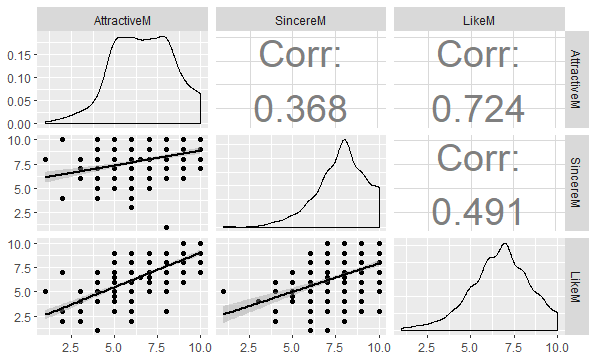
\includegraphics[width=1.0\linewidth]{Images/Rplot_3v}
		\caption{Multivariate plot}
		\label{fig:rplot3v}
	\end{figure}
	
	
	\begin{itemize}
		\item Ta thấy rằng p-value của $F-statistic < 2.2e-16$ điều này có nghĩa là ít nhất 1 biến $x$ thay đổi thì sẽ ảnh hưởng đến output $y$.
		\item R-squared: $59.03\%$ điều này cho thấy mô hình này có square error khá cao do đó khả năng đem đi dự đoán cho quần thể (population) mang lai chinh xác không cao.
		\item Đường thẳng phân tách dữ liệu của ta là: $y = 0.067 + 0.628x_1 + 0.306x_2$
		\item Ta thấy cả AttractiveM và LikeM đều ảnh hưởng đáng kể đến output y. Cụ thế, ta thấy AttractiveM ảnh hưởng nhiều đến LikeM hơn là SincereM (0.628 > 0.306).
		\item Ví dụ: khi AttractiveM tăng 1 thì đầu ra y sẽ tăng 0.067 lần so với khi SincereM tăng 1 thì y chỉ tăng 0.306 lần.
		\item Như đã phân tích ở câu \ref{Cau6} (trang \pageref{Cau6}), ta thấy rằng giữa AttractiveM và LikeM có liên kết dương mạnh ($r_{AL} = 0.724$). Và giữa SincereM và LikeM cũng có liên kết dương trung tính ($r_{SL} = 0.491 \approx 0.5$). Điều này lại một lần nữa khẳng định sự ảnh hưởng của AttractiveM, SincereM lên LikeM là đáng kể.
		\item Thêm vào đó, hệ số tương quan của AttractiveM và SincereM $r_{AS} = 0.368$ không quá mạnh. Điều này cho thấy sự thay đổi của cả 2 không ảnh hưởng đến nhau nhiều.
		\item Ta thấy rằng các scatter plot giữa (AttractiveM, LikeM), (SincereM, LikeM) và (AttractiveM, SincereM) có phần smooth curve màu xám. Phần xám này khá to ở phần đâu khi số lượng point nhỏ và dần về sau phân xám nhỏ đi và biến mất khi số point nhiều hơn.
		\item Các smooth curves này giúp chúng ta thấy được số lượng các liên kết không chắc chắn (uncertain association) với regression line. Sự không chắc chắn này tăng khi dữ liệu quan sát nhỏ và giảm khi dữ liệu quan sát lớn.
		
	\end{itemize}
	
	\section{Tham khảo}
		\label{Tham khao}
		$\lbrack$1$\rbrack$ Lock5withR pdf-file, \href{https://drive.google.com/open?id=1YQN6KA6lvsPVCqWU-4CQJkcxd7248TqD}{Lock5withR}.\\	
		$\lbrack$2$\rbrack$ Quick-R by DataCamp, \href{https://www.statmethods.net/stats/descriptives.html}{Quick-R}\\	
		$\lbrack$3$\rbrack$ Official blog - R Correlation tutorial, \href{https://www.datacamp.com/community/blog/r-correlation-tutorial}{DataCamp-Blog}\\
		$\lbrack$4$\rbrack$ Multiple Linear Regression in R, \href{http://www.sthda.com/english/articles/40-regression-analysis/168-multiple-linear-regression-in-r/}{STHDA - Articles - Regression Analysis}\\
		$\lbrack$5$\rbrack$ Book: Unlocking the power of data, Chapter 2 – Describing Data, \href{https://drive.google.com/open?id=1ilCQevunVvqr4X8OeWca2aswWOwm-YBg}{Robin H. Lock, Patti Frazer Lock, Dennis F. Lock, Kari Lock Morgan, Eric F. Lock - Statistics: Unlocking the Power of Data (2012, Wiley)}
	
\end{document}